\documentclass[11pt,a4paper]{article}

\usepackage[T1]{fontenc}
\usepackage[utf8]{inputenc}
\usepackage{lmodern}
\usepackage[margin=2.3cm]{geometry}
\usepackage{amsmath,amssymb}
\usepackage{booktabs}
\usepackage{array}
\usepackage{tabularx}
\usepackage{enumitem}
\usepackage{xcolor}
\usepackage{tikz}
\usepackage[most]{tcolorbox}
\usepackage{listings}
\usepackage{titlesec}
\usepackage{fancyhdr}
\usepackage[colorlinks=true,linkcolor=blue!50!black,urlcolor=blue!50!black]{hyperref}

\usetikzlibrary{arrows.meta,decorations.pathreplacing,calc}

\definecolor{keyblue}{RGB}{30,80,160}
\definecolor{softblue}{RGB}{232,240,252}
\definecolor{softgreen}{RGB}{232,246,236}
\definecolor{softyellow}{RGB}{253,248,228}
\definecolor{zerored}{RGB}{200,40,40}

\newtcolorbox{keybox}[1][]{colback=softblue,colframe=keyblue,fonttitle=\bfseries,
  boxrule=0.8pt,arc=2pt,left=8pt,right=8pt,top=6pt,bottom=6pt,#1}
\newtcolorbox{analogy}[1][Analogy]{colback=softgreen,colframe=green!45!black,
  fonttitle=\bfseries,title=#1,boxrule=0.6pt,arc=2pt}
\newtcolorbox{example}[1][Example]{colback=softyellow,colframe=orange!70!black,
  fonttitle=\bfseries,title=#1,boxrule=0.6pt,arc=2pt}

\lstset{basicstyle=\ttfamily\small,keywordstyle=\color{keyblue}\bfseries,
  commentstyle=\color{gray}\itshape,frame=single,framesep=4pt,
  backgroundcolor=\color{gray!6},language=Python,showstringspaces=false,
  columns=fullflexible}

\titleformat{\section}{\Large\bfseries\color{keyblue}}{\thesection}{0.8em}{}
\titleformat{\subsection}{\large\bfseries}{\thesubsection}{0.6em}{}

\pagestyle{fancy}
\fancyhf{}
\fancyhead[L]{\small The Riemann Hypothesis, Explained Step by Step}
\fancyhead[R]{\small\thepage}
\renewcommand{\headrulewidth}{0.4pt}

\setlength{\parindent}{0pt}
\setlength{\parskip}{0.55em}

\setcounter{secnumdepth}{0}
\newcommand{\Li}{\operatorname{Li}}

\begin{document}

%==================================================================
\begin{titlepage}
\centering
\vspace*{3cm}
{\Huge\bfseries\color{keyblue} The Riemann Hypothesis\par}
\vspace{0.5cm}
{\LARGE Explained Step by Step\par}
\vspace{1.5cm}
{\large A guide for high school students\par}
\vspace{0.3cm}
{\normalsize You need only basic algebra, exponents, and a bit of curiosity.\par}
\vspace{2cm}

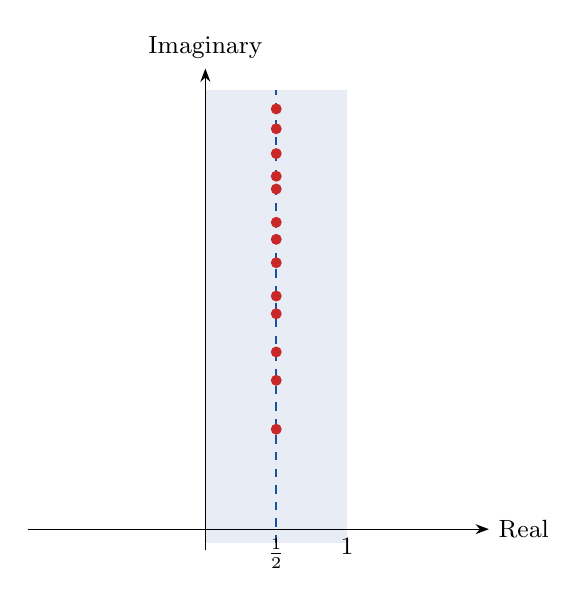
\begin{tikzpicture}[scale=0.9]
  \fill[keyblue!10] (0,-0.2) rectangle (2,6.2);
  \draw[-{Stealth}] (-2.5,0) -- (4,0) node[right]{\small Real};
  \draw[-{Stealth}] (0,-0.3) -- (0,6.5) node[above]{\small Imaginary};
  \draw[dashed,keyblue,thick] (1,-0.2) -- (1,6.2);
  \foreach \y in {1.41,2.10,2.50,3.04,3.29,3.76,4.09,4.33,4.80,4.98,5.30,5.65,5.93}
    \fill[zerored] (1,\y) circle (2.2pt);
  \node[below] at (1,0) {\small $\tfrac12$};
  \node[below] at (2,0) {\small $1$};
\end{tikzpicture}

\vfill
{\large\itshape ``Prime numbers grow like weeds among the natural numbers, seeming to obey no other law than that of chance, but also exhibit stunning regularity.''\par}
\vspace{0.2cm}
{\normalsize --- Don Zagier, mathematician\par}
\vspace{1cm}
\end{titlepage}

\tableofcontents
\newpage

%==================================================================
\section{The One-Sentence Version}

\begin{keybox}
\textbf{The Riemann Hypothesis says that the prime numbers are spread out as evenly and predictably as they possibly could be.} In technical terms: all the ``interesting'' zeros of a special function called the \emph{zeta function} lie on a single straight line.
\end{keybox}

That sentence won't fully make sense yet. By the end of this guide it will. We'll build up to it one small step at a time.

Some background first:
\begin{itemize}[itemsep=2pt]
  \item It was proposed by the German mathematician \textbf{Bernhard Riemann} in \textbf{1859}, in a short paper of about 8 pages titled \emph{``On the Number of Primes Less Than a Given Magnitude.''}
  \item It has been unsolved for more than \textbf{165 years}.
  \item It is one of the seven \textbf{Millennium Prize Problems}. Whoever proves it (or disproves it) wins \textbf{\$1{,}000{,}000} from the Clay Mathematics Institute.
  \item Many mathematicians consider it \textbf{the most important unsolved problem in all of mathematics}.
\end{itemize}

%==================================================================
\section{Step 1: Prime Numbers, the Atoms of Arithmetic}

A \textbf{prime number} is a whole number greater than 1 that can only be divided evenly by \textbf{1 and itself}.

\begin{center}
\begin{tabular}{c l l}
\toprule
Number & Divisors & Prime? \\
\midrule
2 & 1, 2 & Yes \\
3 & 1, 3 & Yes \\
4 & 1, 2, 4 & No ($4 = 2\times 2$) \\
5 & 1, 5 & Yes \\
6 & 1, 2, 3, 6 & No ($6 = 2\times 3$) \\
7 & 1, 7 & Yes \\
9 & 1, 3, 9 & No ($9 = 3\times 3$) \\
11 & 1, 11 & Yes \\
\bottomrule
\end{tabular}
\end{center}

The first primes are:
\[
2,\ 3,\ 5,\ 7,\ 11,\ 13,\ 17,\ 19,\ 23,\ 29,\ 31,\ 37,\ 41,\ 43,\ 47,\ 53,\ 59,\ 61,\ 67,\ 71,\ 73,\ 79,\ 83,\ 89,\ 97,\ \ldots
\]

\subsection*{Why primes are so important}

Every whole number bigger than 1 can be built by \textbf{multiplying primes together}, and there is only \textbf{one way} to do it (ignoring order). This is called the \textbf{Fundamental Theorem of Arithmetic}.
\[
12 = 2\times2\times3, \qquad 30 = 2\times3\times5, \qquad 100 = 2\times2\times5\times5, \qquad 1001 = 7\times11\times13
\]

\begin{analogy}
Just as every substance in chemistry is made of atoms (hydrogen, oxygen, carbon\ldots), every number is made of primes. Primes are the \textbf{atoms of arithmetic}.
\end{analogy}

\subsection*{There are infinitely many primes}

About 2,300 years ago, the Greek mathematician \textbf{Euclid} proved that the primes never run out. His argument is short:
\begin{enumerate}[itemsep=1pt]
  \item Suppose there were only a finite list of primes: $2, 3, 5, \ldots, P$.
  \item Multiply them all together and add 1: $N = (2\times3\times5\times\cdots\times P) + 1$.
  \item Dividing $N$ by any prime on the list leaves a remainder of 1. So none of them divides $N$.
  \item So $N$ is either a new prime itself, or it is made from primes that aren't on the list.
  \item Either way the list was incomplete. Contradiction! So there are infinitely many primes. \hfill$\blacksquare$
\end{enumerate}

%==================================================================
\section{Step 2: Primes Look Random}

If primes are the atoms of numbers, you'd hope they follow a neat pattern. \textbf{They don't seem to.} Look at the \textbf{gaps} between consecutive primes:

\begin{center}
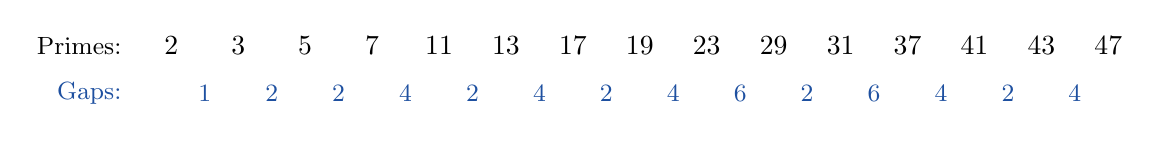
\begin{tikzpicture}[x=0.85cm]
  \foreach \p [count=\i] in {2,3,5,7,11,13,17,19,23,29,31,37,41,43,47}
    \node (p\i) at (\i,0) {\p};
  \foreach \g [count=\i, evaluate=\i as \j using int(\i+1)] in {1,2,2,4,2,4,2,4,6,2,6,4,2,4}
    \node[keyblue,font=\small] at ($(p\i)!0.5!(p\j)+(0,-0.6)$) {\g};
  \node[left] at (0.4,0) {\small Primes:};
  \node[left,keyblue] at (0.4,-0.6) {\small Gaps:};
\end{tikzpicture}
\end{center}

The gaps jump around unpredictably. Sometimes primes come in pairs that are just 2 apart (like 11 and 13, or 41 and 43). These are called \textbf{twin primes}. Other times there are long deserts with no primes at all. For example, there are \textbf{no primes} between 113 and 127.

You can even build arbitrarily long stretches with no primes. The numbers
\[
5!+2,\quad 5!+3,\quad 5!+4,\quad 5!+5 \qquad (\text{that's } 122,\ 123,\ 124,\ 125)
\]
are all composite, because $5! = 120$ is divisible by 2, 3, 4 and 5. Use $1{,}000{,}001!$ instead and you get a million composite numbers in a row.

There is \textbf{no simple formula} that spits out the $n$-th prime. Primes look almost like they were sprinkled randomly along the number line.

\begin{keybox}
\textbf{The big question:} Is there \emph{any} hidden order in the primes?
\end{keybox}

%==================================================================
\section{Step 3: Counting Primes, and a Surprising Pattern}

Instead of predicting each individual prime (too hard), mathematicians asked an easier question:

\begin{keybox}
\textbf{How many primes are there up to a number $x$?}
\end{keybox}

This count is written $\pi(x)$. (It's the Greek letter ``pi'', but here it has \emph{nothing} to do with $3.14159\ldots$ It's just a name.)

\begin{example}
\begin{itemize}[itemsep=1pt,leftmargin=*]
  \item $\pi(10) = 4$, because the primes up to 10 are 2, 3, 5, 7.
  \item $\pi(20) = 8$, because the primes up to 20 are 2, 3, 5, 7, 11, 13, 17, 19.
  \item $\pi(100) = 25$.
\end{itemize}
\end{example}

Here is a bigger table:

\begin{center}
\begin{tabular}{r r c}
\toprule
$x$ & $\pi(x)$ = primes up to $x$ & Fraction of numbers that are prime \\
\midrule
10 & 4 & 1 in 2.5 \\
100 & 25 & 1 in 4 \\
1{,}000 & 168 & 1 in 6 \\
10{,}000 & 1{,}229 & 1 in 8.1 \\
100{,}000 & 9{,}592 & 1 in 10.4 \\
1{,}000{,}000 & 78{,}498 & 1 in 12.7 \\
1{,}000{,}000{,}000 & 50{,}847{,}534 & 1 in 19.7 \\
\bottomrule
\end{tabular}
\end{center}

\textbf{Notice:} primes get \emph{rarer} as numbers get bigger. But they thin out in a very \textbf{regular} way. Each time you multiply $x$ by 10, the ``1 in \underline{\hspace{1em}}'' number goes up by about \textbf{2.3}.

\subsection*{Gauss's brilliant guess}

Around 1792, a 15-year-old \textbf{Carl Friedrich Gauss} noticed this pattern. The number 2.3 is approximately $\ln(10)$, the \emph{natural logarithm} of 10. (On a calculator, ``ln'' is the button next to ``log''.) Gauss guessed:

\begin{keybox}
Near a number $x$, about 1 in every $\ln(x)$ numbers is prime. So the number of primes up to $x$ should be roughly
\[
\pi(x) \approx \frac{x}{\ln(x)}.
\]
\end{keybox}

Let's check:

\begin{center}
\begin{tabular}{r r r r}
\toprule
$x$ & Actual $\pi(x)$ & Guess $x/\ln(x)$ & Better guess $\Li(x)$ \\
\midrule
1{,}000 & 168 & 145 & 178 \\
1{,}000{,}000 & 78{,}498 & 72{,}382 & 78{,}628 \\
1{,}000{,}000{,}000 & 50{,}847{,}534 & 48{,}254{,}942 & 50{,}849{,}235 \\
\bottomrule
\end{tabular}
\end{center}

The guess $x/\ln(x)$ is in the right ballpark. Gauss also found a \textbf{better} version called the \textbf{logarithmic integral}:
\[
\Li(x) = \int_2^x \frac{dt}{\ln t}.
\]
You can think of it as ``adding up the chance $1/\ln(t)$ of each number $t$ being prime, for every $t$ from 2 to $x$.'' It's amazingly accurate: off by only about 1,700 out of 50 million!

This result (that the ratio of $\pi(x)$ to $x/\ln(x)$ gets closer and closer to 1) was finally \emph{proven} in 1896 and is called the \textbf{Prime Number Theorem}.

\subsection*{The real question}

$\Li(x)$ is a great estimate, but it's not perfect. There is always some \textbf{error}:
\[
\text{error} = \pi(x) - \Li(x).
\]

\begin{keybox}
\textbf{How big can this error get?}
\end{keybox}

If the error is small, primes are ``well-behaved'': they follow the predicted pattern closely. If the error can be huge, then primes can clump together or spread out in wild ways.

\textbf{The Riemann Hypothesis is exactly the claim that this error is as small as it can possibly be.} To see why, we need Riemann's tool: the zeta function.

%==================================================================
\section{Step 4: Adding Up Infinitely Many Fractions}

Before we meet the zeta function, let's play with infinite sums.

\subsection*{Example A: A sum that blows up}
\[
1 + \frac12 + \frac13 + \frac14 + \frac15 + \cdots
\]
This is called the \textbf{harmonic series}. Each term gets smaller, but the total \textbf{grows forever} (just very slowly). After 1 million terms, the sum is only about 14.4. But it never stops growing. Why? Group the terms:
\[
1 + \frac12 + \underbrace{\left(\frac13+\frac14\right)}_{>\,\frac12} + \underbrace{\left(\frac15+\frac16+\frac17+\frac18\right)}_{>\,\frac12} + \cdots
\]
Each group is bigger than $\frac12$, and there are infinitely many groups. So the total is infinite.

\subsection*{Example B: A sum that settles down}

Now square each denominator:
\[
1 + \frac14 + \frac19 + \frac1{16} + \frac1{25} + \cdots
\]

\begin{center}
\begin{tabular}{r l}
\toprule
Terms added & Running total \\
\midrule
1 & 1.0000 \\
2 & 1.2500 \\
3 & 1.3611 \\
4 & 1.4236 \\
10 & 1.5498 \\
100 & 1.6350 \\
1{,}000 & 1.6439 \\
$\infty$ & \textbf{1.6449\ldots} \\
\bottomrule
\end{tabular}
\end{center}

This one \textbf{converges}: it settles on a finite value. In 1734, \textbf{Leonhard Euler} shocked the world by showing the exact answer is:
\[
1 + \frac14 + \frac19 + \frac1{16} + \cdots = \frac{\pi^2}{6} \approx 1.6449
\]
Yes, that's the \emph{real} $\pi = 3.14159\ldots$, the circle number, showing up in a sum about whole numbers. Math is full of surprises like this.

%==================================================================
\section{Step 5: The Zeta Function}

Notice the pattern in the two sums above. The only difference is the \textbf{exponent} on the denominators:
\begin{itemize}[itemsep=1pt]
  \item Exponent 1: $\ 1 + \frac1{2^1} + \frac1{3^1} + \frac1{4^1} + \cdots$ \quad (blows up)
  \item Exponent 2: $\ 1 + \frac1{2^2} + \frac1{3^2} + \frac1{4^2} + \cdots$ \quad ($=\pi^2/6$)
\end{itemize}

Let's make the exponent a variable, $s$. That gives us the \textbf{zeta function} ($\zeta$ is the Greek letter ``zeta''):

\begin{keybox}
\[
\zeta(s) = \frac1{1^s} + \frac1{2^s} + \frac1{3^s} + \frac1{4^s} + \frac1{5^s} + \cdots = \sum_{n=1}^{\infty} \frac{1}{n^s}
\]
\end{keybox}

\textbf{A function is a machine:} you feed in a number $s$, and it gives you back a number $\zeta(s)$.

\begin{center}
\begin{tabular}{c l l}
\toprule
Input $s$ & $\zeta(s)$ & Notes \\
\midrule
1 & $\infty$ & The harmonic series, which blows up \\
2 & $\pi^2/6 \approx 1.6449$ & Euler's famous result \\
3 & $\approx 1.2021$ & Called Ap\'ery's constant \\
4 & $\pi^4/90 \approx 1.0823$ & \\
10 & $\approx 1.0010$ & Terms shrink so fast the sum is barely above 1 \\
\bottomrule
\end{tabular}
\end{center}

The sum only works (converges) when \textbf{$s$ is bigger than 1}. Keep that in mind. It matters in Step 8.

%==================================================================
\section{Step 6: Euler's Magic Link Between Zeta and Primes}

So far, the zeta function looks like it's about \emph{all} whole numbers. What does it have to do with primes?

Euler discovered something amazing. The zeta function can also be written as a \textbf{product over only the primes}:
\[
\zeta(s) = \frac{1}{1-\frac{1}{2^s}} \times \frac{1}{1-\frac{1}{3^s}} \times \frac{1}{1-\frac{1}{5^s}} \times \frac{1}{1-\frac{1}{7^s}} \times \frac{1}{1-\frac{1}{11^s}} \times \cdots = \prod_{p \text{ prime}} \frac{1}{1-p^{-s}}
\]
One factor for \textbf{every prime}, and nothing else.

\subsection*{Why is this true? (A peek under the hood)}

Remember the geometric series: $\dfrac{1}{1-r} = 1 + r + r^2 + r^3 + \cdots$. So each factor expands like this:
\begin{align*}
\frac{1}{1-\frac{1}{2^s}} &= 1 + \frac1{2^s} + \frac1{4^s} + \frac1{8^s} + \cdots && \text{(powers of 2)}\\[4pt]
\frac{1}{1-\frac{1}{3^s}} &= 1 + \frac1{3^s} + \frac1{9^s} + \frac1{27^s} + \cdots && \text{(powers of 3)}
\end{align*}
and so on for $5, 7, 11, \ldots$

When you multiply all these together, you pick one term from each bracket. For example, to get $\frac{1}{12^s}$:
\begin{itemize}[itemsep=1pt]
  \item From the ``2'' bracket pick $\frac1{4^s}$ (since $4 = 2^2$).
  \item From the ``3'' bracket pick $\frac1{3^s}$.
  \item From every other bracket pick $1$.
\end{itemize}
Result: $\frac1{4^s}\times\frac1{3^s} = \frac1{12^s}$.

Because every number has \textbf{exactly one} prime factorization (Step 1!), \textbf{every} $\frac1{n^s}$ appears \textbf{exactly once}. So the product equals the sum.

\begin{keybox}
\textbf{Key takeaway:} The zeta function is a bridge. One side is all the whole numbers (easy to understand). The other side is the primes (mysterious). Studying $\zeta(s)$ lets us study primes.
\end{keybox}

As a bonus, this gives another proof that there are infinitely many primes. At $s = 1$ the sum is infinite. A \emph{finite} product could never be infinite, so there must be infinitely many prime factors.

%==================================================================
\section{Step 7: A Quick Tour of Complex Numbers}

Riemann's big idea was to plug \textbf{complex numbers} into the zeta function. Here's a quick, painless introduction.

\subsection*{The imaginary number $i$}

There's no ordinary (real) number whose square is $-1$. Mathematicians simply \textbf{invented one} and called it $i$:
\[
i^2 = -1.
\]

\subsection*{Complex numbers}

A \textbf{complex number} is a combination of a real part and an imaginary part:
\[
s = a + b\,i
\]
Examples: $3 + 2i$, \ $-1 + 5i$, \ $0.5 + 14.13i$, \ $7$ (which is $7 + 0i$).

\subsection*{Picture them as points on a map}

Think of the complex numbers as a \textbf{2D map} (called the \textbf{complex plane}). Left--right position is the \textbf{real part} $a$; up--down position is the \textbf{imaginary part} $b$.

\begin{center}
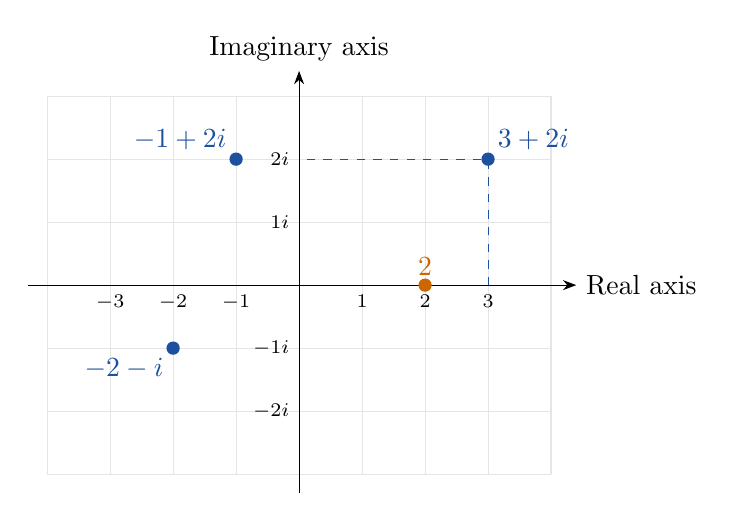
\begin{tikzpicture}[scale=0.8]
  \draw[step=1,gray!20] (-4,-3) grid (4,3);
  \draw[-{Stealth}] (-4.3,0) -- (4.4,0) node[right]{Real axis};
  \draw[-{Stealth}] (0,-3.3) -- (0,3.4) node[above]{Imaginary axis};
  \foreach \x in {-3,-2,-1,1,2,3} \node[below,font=\scriptsize] at (\x,0) {$\x$};
  \foreach \y in {-2,-1,1,2} \node[left,font=\scriptsize] at (0,\y) {$\y i$};
  \fill[keyblue] (3,2) circle (3pt) node[above right]{$3+2i$};
  \fill[keyblue] (-2,-1) circle (3pt) node[below left]{$-2-i$};
  \fill[keyblue] (-1,2) circle (3pt) node[above left]{$-1+2i$};
  \fill[orange!80!black] (2,0) circle (3pt) node[above]{$2$};
  \draw[dashed,keyblue] (3,0) -- (3,2) -- (0,2);
\end{tikzpicture}
\end{center}

Ordinary numbers like $2$, $3$, $-5$ just sit on the horizontal line. Complex numbers fill up the whole plane.

\textbf{Why bother?} Many problems become \emph{easier} once you allow complex numbers. It's like solving a maze by looking at it from above instead of from inside.

%==================================================================
\section{Step 8: Riemann Extends Zeta to the Whole Plane}

Remember: the sum $1 + \frac1{2^s} + \frac1{3^s} + \cdots$ only makes sense when the real part of $s$ is \textbf{greater than 1}. On our map, that's only the shaded region on the right:

\begin{center}
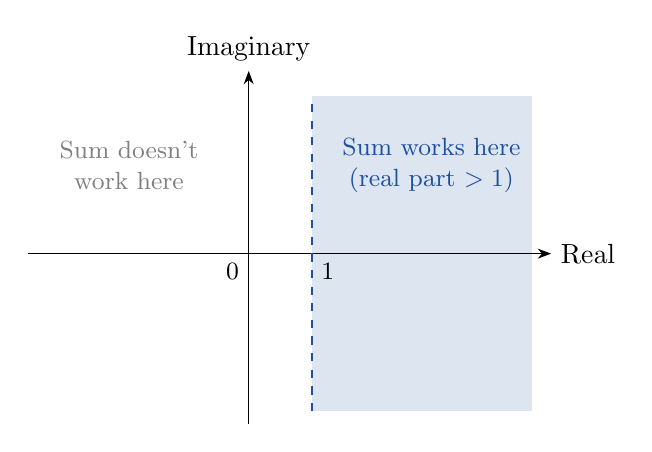
\begin{tikzpicture}[scale=0.8]
  \fill[keyblue!15] (1,-2.5) rectangle (4.5,2.5);
  \draw[-{Stealth}] (-3.5,0) -- (4.8,0) node[right]{Real};
  \draw[-{Stealth}] (0,-2.7) -- (0,2.9) node[above]{Imaginary};
  \draw[dashed,keyblue,thick] (1,-2.5) -- (1,2.5);
  \node[below left,font=\small] at (0,0) {$0$};
  \node[below right,font=\small] at (1,0) {$1$};
  \node[keyblue,align=center,font=\small] at (2.9,1.4) {Sum works here\\(real part $>1$)};
  \node[gray,align=center,font=\small] at (-1.9,1.4) {Sum doesn't\\work here};
\end{tikzpicture}
\end{center}

Riemann found a way to \textbf{extend} the zeta function to the \textbf{entire} complex plane (except the single point $s = 1$, where it blows up). This is called \textbf{analytic continuation}.

\begin{analogy}[Analogy: finishing a drawing]
Imagine someone draws the right half of a perfectly smooth curve and asks you to finish it. For special ``smooth'' functions in complex math, there is \textbf{only one possible way} to continue the drawing. Riemann found that unique continuation for zeta.
\end{analogy}

On the extended function, some strange-looking values appear, like:
\[
\zeta(0) = -\frac12, \qquad \zeta(-1) = -\frac1{12}.
\]
\textbf{Important:} This does \emph{not} mean that $1 + 2 + 3 + 4 + \cdots$ ``really'' equals $-\frac1{12}$. The original sum doesn't work there at all. These are values of the \emph{extended} function, which is defined in a different way in that region.

Riemann also discovered a beautiful \textbf{mirror symmetry}: the value of $\zeta$ at $s$ is tied to its value at $1 - s$. This symmetry is centered on the vertical line where the real part equals $\tfrac12$. Keep an eye on that line!

%==================================================================
\section{Step 9: Zeros, the Places Where Zeta Equals 0}

A \textbf{zero} of a function is an input that makes the output equal \textbf{0}.

\begin{example}[Simple example]
For $f(x) = x^2 - 4$, the zeros are $x = 2$ and $x = -2$, since $2^2 - 4 = 0$ and $(-2)^2 - 4 = 0$.

Zeros are incredibly useful. If you know all the zeros of a polynomial, you basically know the whole polynomial. For example, zeros at $2$ and $-2$ give $f(x) = (x-2)(x+2)$.
\end{example}

\subsection*{The zeros of zeta come in two kinds}

\textbf{1. Trivial zeros (the boring ones).} $\zeta(s) = 0$ at every \textbf{negative even number}:
\[
s = -2,\ -4,\ -6,\ -8,\ \ldots
\]
These are well understood and easy to find. Nobody worries about them.

\textbf{2. Non-trivial zeros (the mysterious ones).} All the \emph{other} zeros are complex numbers. Riemann proved they must all lie in a vertical strip between real part 0 and real part 1. This is called the \textbf{critical strip}.

Here are the first few non-trivial zeros. They come in mirror pairs, above and below the real axis; these are the ones above:

\begin{center}
\begin{tabular}{c l}
\toprule
\# & Zero \\
\midrule
1st & $\mathbf{0.5} + 14.1347\,i$ \\
2nd & $\mathbf{0.5} + 21.0220\,i$ \\
3rd & $\mathbf{0.5} + 25.0109\,i$ \\
4th & $\mathbf{0.5} + 30.4249\,i$ \\
5th & $\mathbf{0.5} + 32.9351\,i$ \\
\bottomrule
\end{tabular}
\end{center}

Do you notice something? \textbf{Every single one has real part exactly 0.5 (one half).}

%==================================================================
\section{Step 10: The Riemann Hypothesis Itself}

Now we can finally state it:

\begin{tcolorbox}[colback=keyblue!8,colframe=keyblue,boxrule=1.5pt,arc=3pt,
  title=\Large\bfseries The Riemann Hypothesis,fonttitle=\color{white},halign title=center]
\Large\centering
Every non-trivial zero of the zeta function has real part equal to $\tfrac12$.
\end{tcolorbox}

In other words, all the interesting zeros lie on a single vertical line through $\frac12$, called the \textbf{critical line}:

\begin{center}
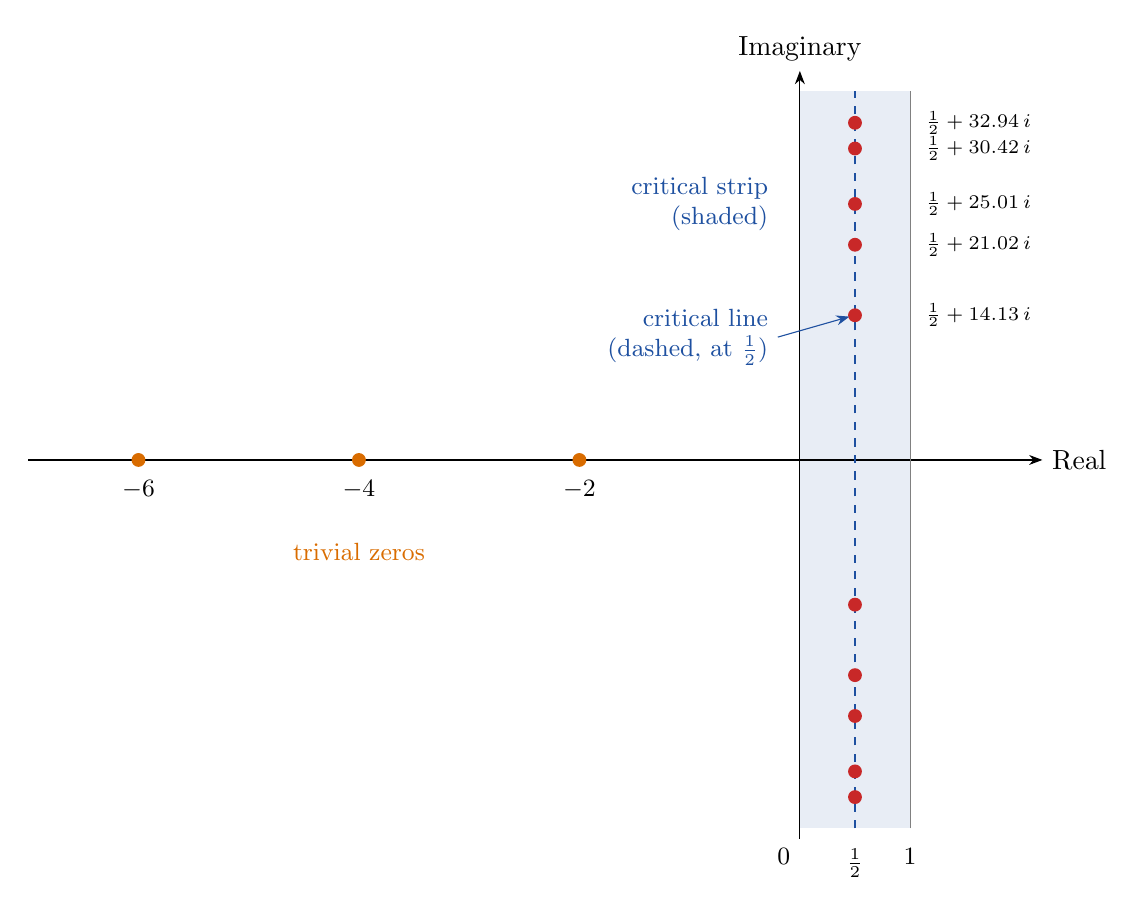
\begin{tikzpicture}[x=1.4cm,y=0.13cm]
  % critical strip
  \fill[keyblue!10] (0,-36) rectangle (1,36);
  \draw[-{Stealth}] (-7,0) -- (2.2,0) node[right]{Real};
  \draw[-{Stealth}] (0,-37) -- (0,38) node[above]{Imaginary};
  \draw[keyblue,thick,dashed] (0.5,-36) -- (0.5,36);
  \draw[gray] (1,-36) -- (1,36);
  % zeros
  \foreach \y/\lab in {14.1347/14.13,21.0220/21.02,25.0109/25.01,30.4249/30.42,32.9351/32.94}{
    \fill[zerored] (0.5,\y) circle (2.5pt);
    \fill[zerored] (0.5,-\y) circle (2.5pt);
    \node[right,font=\scriptsize] at (1.05,\y) {$\tfrac12 + \lab\, i$};
  }
  % trivial zeros
  \foreach \x in {-2,-4,-6}{
    \fill[orange!85!black] (\x,0) circle (2.5pt);
    \node[below,font=\small] at (\x,-1) {$\x$};
  }
  \node[orange!85!black,font=\small,align=center] at (-4,-9) {trivial zeros};
  \node[below,font=\small] at (0.5,-37) {$\tfrac12$};
  \node[below,font=\small] at (1,-37) {$1$};
  \node[below left,font=\small] at (0,-37) {$0$};
  \node[keyblue,font=\small,align=right,left] at (-0.2,25) {critical strip\\(shaded)};
  \node[keyblue,font=\small,align=right,left] at (-0.2,12) {critical line\\(dashed, at $\tfrac12$)};
  \draw[keyblue,-{Stealth}] (-0.2,12) -- (0.45,14);
\end{tikzpicture}
\end{center}

The hypothesis says the red dots \textbf{never} wander off the middle line, not even once, no matter how far up you go.

\begin{analogy}[Analogy: a tightrope]
Picture an infinitely tall tightrope stretched straight up. Riemann claimed that infinitely many acrobats (the zeros) are all standing \textbf{exactly on the rope}. We've checked trillions of them, and every one is on the rope. But we can't check all infinitely many by hand. We need a \textbf{proof} that \emph{none} can ever fall off.
\end{analogy}

%==================================================================
\section{Step 11: Why the Zeros Control the Primes}

This is the most beautiful part. Why should zeros on a line in the complex plane have anything to do with counting primes?

Riemann found an \textbf{exact formula} for counting primes. Very roughly, it says:
\[
\big(\text{prime count up to } x\big) \;=\; \big(\text{smooth main estimate}\big) \;-\; \sum_{\text{zeros}} \big(\text{a wave for each zero}\big)
\]

\begin{analogy}[Analogy: music]
Think of the prime count $\pi(x)$ as a \textbf{staircase}. It's flat, then jumps up by 1 at each prime. It's a jagged, irregular shape.

Now think of how a music producer builds a complicated sound out of simple pure tones (sine waves) added together. Riemann showed you can do the \textbf{same thing} with the prime staircase.
\end{analogy}

\begin{center}
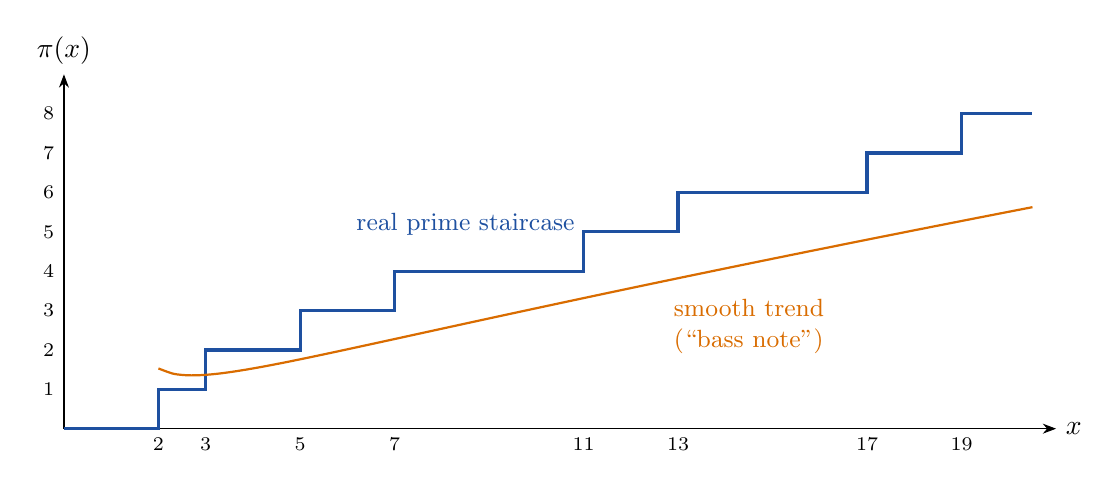
\begin{tikzpicture}[x=0.6cm,y=0.5cm]
  \draw[-{Stealth}] (0,0) -- (21,0) node[right]{$x$};
  \draw[-{Stealth}] (0,0) -- (0,9) node[above]{$\pi(x)$};
  \foreach \y in {1,...,8} \node[left,font=\scriptsize] at (0,\y) {\y};
  % staircase
  \draw[keyblue,very thick]
    (0,0) -- (2,0) -- (2,1) -- (3,1) -- (3,2) -- (5,2) -- (5,3) -- (7,3) -- (7,4)
    -- (11,4) -- (11,5) -- (13,5) -- (13,6) -- (17,6) -- (17,7) -- (19,7) -- (19,8) -- (20.5,8);
  \foreach \p in {2,3,5,7,11,13,17,19} \node[below,font=\scriptsize] at (\p,0) {\p};
  % smooth Li(x)-Li(2) approx curve
  \draw[orange!85!black,thick,domain=2:20.5,samples=60,smooth]
    plot (\x,{1.05*(\x)/ln(\x) - 1.5});
  \node[orange!85!black,font=\small,align=left] at (14.5,2.6) {smooth trend\\(``bass note'')};
  \node[keyblue,font=\small] at (8.5,5.2) {real prime staircase};
\end{tikzpicture}
\end{center}

\begin{itemize}[itemsep=2pt]
  \item The \textbf{smooth curve} $\Li(x)$ gives the general rising trend (the ``bass note'').
  \item Each \textbf{non-trivial zero} contributes one \textbf{wave} (a ``harmonic'') that adds a little wiggle.
  \item Add up all the waves from all the zeros, and you rebuild the \textbf{exact} jagged staircase, jumping at precisely the primes!
\end{itemize}

\subsection*{What each zero controls}

\begin{itemize}[itemsep=2pt]
  \item The zero's \textbf{height} (imaginary part, like $14.13$) sets \textbf{how fast} its wave wiggles. That's its \emph{frequency} or pitch.
  \item The zero's \textbf{real part} (like $\tfrac12$) sets \textbf{how loud} that wave gets as $x$ grows. That's its \emph{volume}.
\end{itemize}

A zero with real part $\sigma$ (the Greek letter sigma) produces a wave whose size grows like $x^{\sigma}$.
\begin{itemize}[itemsep=2pt]
  \item If every zero has real part $\frac12$, every wave grows only like $x^{1/2} = \sqrt{x}$.
  \item If some zero had real part, say, $0.9$, its wave would grow like $x^{0.9}$, which is much louder, and it would make the primes much more irregular.
\end{itemize}

Because of the mirror symmetry, zeros pair up around the line $\frac12$ (a zero at $0.9 + bi$ would force a partner at $0.1 + bi$). So $\frac12$ is the \emph{best possible} case. That gives us the precise meaning of the Riemann Hypothesis:

\begin{keybox}
\textbf{The Riemann Hypothesis} $\iff$ \textbf{The error in counting primes is about as small as possible}, roughly $\sqrt{x}$ (times a small logarithm factor). In symbols, if RH is true then
\[
\big|\pi(x) - \Li(x)\big| \;\le\; \frac{1}{8\pi}\,\sqrt{x}\,\ln(x) \qquad \text{for all } x \ge 2657.
\]
\end{keybox}

\begin{example}[A concrete example: one billion]
At $x = 1{,}000{,}000{,}000$:
\begin{itemize}[itemsep=1pt,leftmargin=*]
  \item $\sqrt{x} \approx 31{,}623$ and $\ln(x) \approx 20.7$.
  \item The RH bound allows an error up to about $\dfrac{1}{25.1}\times 31{,}623 \times 20.7 \approx \mathbf{26{,}000}$.
  \item The actual error is $|50{,}847{,}534 - 50{,}849{,}235| \approx \mathbf{1{,}700}$.
\end{itemize}
It fits comfortably within the bound, just as RH predicts. The ``random-looking'' primes are actually tightly controlled.
\end{example}

\subsection*{Coin-flip comparison}

If you flip a fair coin $x$ times, the number of heads is usually within about $\sqrt{x}$ of $x/2$. The Riemann Hypothesis says primes deviate from their expected count about as little as \textbf{random coin flips} would. They are as ``fair'' and balanced as randomness allows: no weird conspiracies, no huge clumps.

%==================================================================
\section{Step 12: What We Know, and What We Don't}

\subsection*{What has been proven}

\begin{itemize}[itemsep=2pt]
  \item \textbf{1859:} Riemann proves all non-trivial zeros lie in the critical strip (real part between 0 and 1) and states the hypothesis.
  \item \textbf{1896:} Hadamard and de la Vall\'ee Poussin prove there are \textbf{no zeros on the line real part $=1$}. That's exactly what's needed to prove the \textbf{Prime Number Theorem}.
  \item \textbf{1914:} G.\,H.\ Hardy proves that \textbf{infinitely many} zeros lie on the critical line. (But not that \emph{all} of them do.)
  \item \textbf{1989:} Brian Conrey proves that \textbf{at least 40\%} of the non-trivial zeros are on the critical line.
  \item \textbf{Computers:} More than \textbf{10 trillion} zeros have been computed. \textbf{Every single one} is on the critical line.
\end{itemize}

\subsection*{What remains unknown}

\begin{itemize}[itemsep=2pt]
  \item Nobody has proven that \textbf{100\%} of the zeros are on the line.
  \item Nobody has even proven that zeros can't get arbitrarily close to the edge of the strip.
  \item 10 trillion examples is \textbf{not} a proof. In math, a pattern can hold for a huge number of cases and still fail eventually.
\end{itemize}

\begin{example}[A cautionary tale]
For all values ever computed, $\pi(x) < \Li(x)$. People guessed this was always true. But in 1914, J.\,E.\ Littlewood proved that $\pi(x)$ eventually becomes \emph{bigger} than $\Li(x)$. The first time this happens is thought to be near $10^{316}$ (a 1 followed by 316 zeros), a number far too large for any computer to reach. So checking lots of cases isn't enough; we need proof.
\end{example}

%==================================================================
\section{Step 13: Why It Matters}

\subsection*{1. Thousands of results depend on it}
Mathematicians have proven \textbf{hundreds of theorems} that begin with ``\emph{Assuming the Riemann Hypothesis is true, then\ldots}''. If RH is proven, all of them become true instantly. If it's false, many collapse.

\subsection*{2. Understanding the primes}
RH would give us the best possible understanding of how primes are distributed. For example, it would guarantee that there is always a prime reasonably close to any large number $x$ (within roughly $\sqrt{x}\,\ln x$ of it).

\subsection*{3. Cryptography and computer security}
Internet security (like the RSA encryption behind HTTPS) relies on large primes and on how hard it is to break big numbers into prime factors. Proving RH \textbf{would not break encryption}. That's a common myth. But many algorithms for finding and testing primes are known to run fast \textbf{if RH is true}.

\subsection*{4. Surprising connection to physics}
In the 1970s, mathematician \textbf{Hugh Montgomery} found a formula for how the spacing between zeta zeros behaves. Physicist \textbf{Freeman Dyson} recognized it immediately: it was the \textbf{same formula} that describes the energy levels of heavy atomic nuclei in quantum physics! Nobody fully understands why primes and quantum physics seem linked. Some researchers hope that finding the ``quantum system'' behind the zeros could lead to a proof.

\subsection*{5. The million-dollar prize}
The Clay Mathematics Institute offers \textbf{\$1{,}000{,}000} for a correct proof. Many famous mathematicians have tried; none have succeeded. The mathematician David Hilbert reportedly said that if he woke up after sleeping for 1,000 years, his first question would be: \emph{``Has the Riemann Hypothesis been proven?''}

%==================================================================
\section{Summary: The Whole Story on One Page}

\begin{center}
\renewcommand{\arraystretch}{1.25}
\begin{tabularx}{\textwidth}{c l X}
\toprule
Step & Idea & One-line explanation \\
\midrule
1 & Primes & Numbers divisible only by 1 and themselves; the building blocks of all numbers \\
2 & Randomness & Primes look scattered and unpredictable \\
3 & Counting & $\pi(x)$ counts primes up to $x$; it's close to $\Li(x)$, but how close? \\
4 & Infinite sums & Some infinite sums settle on a value: $1 + \frac14 + \frac19 + \cdots = \frac{\pi^2}{6}$ \\
5 & Zeta function & $\zeta(s) = 1 + \frac1{2^s} + \frac1{3^s} + \cdots$ \\
6 & Euler product & $\zeta(s)$ can also be written using only primes: a bridge to the primes \\
7 & Complex numbers & Numbers like $a + bi$, pictured as points on a 2D map \\
8 & Extension & Riemann extends $\zeta$ to the whole complex map \\
9 & Zeros & Places where $\zeta(s) = 0$; trivial ones at $-2, -4, \ldots$; mysterious ones in the strip \\
10 & \textbf{The Hypothesis} & \textbf{All mysterious zeros have real part exactly $\tfrac12$} \\
11 & Link to primes & Each zero adds a ``wave'' to the prime count; real part $\frac12$ means the smallest possible error ($\approx\sqrt{x}$) \\
12 & Status & 10+ trillion zeros checked, all on the line; still no proof \\
13 & Importance & Hundreds of theorems depend on it; \$1M prize; strange links to physics \\
\bottomrule
\end{tabularx}
\end{center}

\begin{keybox}[title=The core idea in plain words]
Prime numbers look random. But Riemann discovered they are secretly controlled by a hidden set of points (the zeros of the zeta function). Like notes in a piece of music, these zeros decide how the primes are arranged. The Riemann Hypothesis says all these notes sit on one perfect line. If true, the primes are as orderly as anything random-looking could possibly be. \textbf{No one has been able to prove it, yet.}
\end{keybox}

%==================================================================
\section{Try It Yourself}

\begin{enumerate}[itemsep=6pt]
  \item \textbf{Count primes:} Find $\pi(50)$.\\
  \emph{Answer: 15. The primes are 2, 3, 5, 7, 11, 13, 17, 19, 23, 29, 31, 37, 41, 43, 47.}

  \item \textbf{Check Gauss's guess:} Compute $50/\ln(50)$ on a calculator. How close is it to $\pi(50)$?\\
  \emph{Answer: about 12.8, a bit low but in the right range.}

  \item \textbf{Build $\zeta(2)$ by hand:} Add $1 + \frac14 + \frac19 + \frac1{16} + \frac1{25} + \frac1{36}$. Compare with $\frac{\pi^2}{6} \approx 1.6449$.\\
  \emph{Answer: $\approx 1.4914$. You're getting there slowly!}

  \item \textbf{Euler product check:} Multiply just the first three prime factors for $s = 2$:
  \[
  \frac{1}{1-\frac14}\times\frac{1}{1-\frac19}\times\frac{1}{1-\frac1{25}}.
  \]
  \emph{Answer: $\frac43\times\frac98\times\frac{25}{24} = 1.5625$. Adding more primes gets you closer to 1.6449.}

  \item \textbf{Complex numbers:} Compute $(1+i)^2$. Remember that $i^2 = -1$.\\
  \emph{Answer: $1 + 2i + i^2 = 2i$.}

  \item \textbf{Code it (optional):} If you know Python, try this:
\begin{lstlisting}
import math

def zeta(s, terms=100000):
    return sum(1 / n**s for n in range(1, terms + 1))

print(zeta(2), math.pi**2 / 6)   # both about 1.6449

def count_primes(x):
    sieve = [True] * (x + 1)
    sieve[0] = sieve[1] = False
    for i in range(2, int(x**0.5) + 1):
        if sieve[i]:
            for j in range(i * i, x + 1, i):
                sieve[j] = False
    return sum(sieve)

for x in [100, 1000, 10000, 100000]:
    print(x, count_primes(x), round(x / math.log(x)))
\end{lstlisting}
\end{enumerate}

%==================================================================
\section{Glossary}

\begin{center}
\renewcommand{\arraystretch}{1.2}
\begin{tabularx}{\textwidth}{>{\bfseries}l X}
\toprule
\normalfont\textbf{Term} & \textbf{Meaning} \\
\midrule
Prime number & A whole number $>1$ divisible only by 1 and itself \\
$\boldsymbol{\pi(x)}$ & The number of primes less than or equal to $x$ \\
$\boldsymbol{\ln(x)}$ & The natural logarithm; $\ln(10) \approx 2.3$ \\
$\boldsymbol{\Li(x)}$ & The logarithmic integral; a very accurate estimate of $\pi(x)$ \\
Prime Number Theorem & Proven fact that $\pi(x) \approx x/\ln(x)$ for large $x$ \\
Converge & An infinite sum settles on a finite value \\
Zeta function $\boldsymbol{\zeta(s)}$ & $\zeta(s) = 1 + \frac1{2^s} + \frac1{3^s} + \cdots$, extended by Riemann to all complex $s \ne 1$ \\
Euler product & Writing $\zeta(s)$ as a product with one factor per prime \\
$\boldsymbol{i}$ & The imaginary unit, with $i^2 = -1$ \\
Complex number & A number $a + bi$, shown as a point on a 2D plane \\
Analytic continuation & The unique smooth way to extend a function beyond where its formula works \\
Zero of a function & An input where the function outputs 0 \\
Trivial zeros & The zeros of $\zeta$ at $-2, -4, -6, \ldots$ \\
Non-trivial zeros & The complex zeros of $\zeta$ inside the critical strip \\
Critical strip & The vertical band of the complex plane where the real part is between 0 and 1 \\
Critical line & The vertical line where the real part $= \frac12$ \\
Riemann Hypothesis & The claim that every non-trivial zero lies on the critical line \\
\bottomrule
\end{tabularx}
\end{center}

\end{document}
